
\section{Kubernetes}

Jméno Kubernetes pochází z Řecka a znamená to kormidelník. Projekt zložili Joe Beda, Brendan Burns, a Craig McLuckie,ke kterým se rychle připojili inženýři z Googlu, jako Brian Grant a Tim Hockin. Software byl vydán v roce 2014.

Kontejnery jsou perfektní způsob, jak vytvářet aplikace tak, aby byly lehce rozšiřitelné a dobře spravovatelné. Kubernetes nám následné pomáhá k jejich nasazení a škálování. Co všechno tedy Kubernetes dokáží:

%https://kubernetes.io/docs/concepts/overview/what-is-kubernetes/

\begin{itemize}
  	\item \textbf{Service discovery and load balancing}: Kubernetes propojují kontejnery zkrze DNS a nebo jejich IP adresy. Pokud na jeden 	kontejner jde mnoho požadavků, přesměrují tyto požadavky na jiný a tímto způsobem balancují provoz a zajišťují stabilitu aplikace.
	\item \textbf{Orchestrace úložiště}: Dovolují automaticky připojovat vzdálené nebo lokální úložiště do klastru a zajistit tak konzistenci dat, zálohu a vysokou dostupnost z více míst.
  	\item \textbf{Automated rollouts and rollbacks}: Můžeme popsat požadovaný stav pro naše nasazené kontejnery pomocí Kubernetes a ty automaticky a s kontrolou zajistí tento stav. Můžeme například automatizovat vytváření nových kontejnerů, smazání starých a převzetí všech zdrojů jako jsou data a další novým kontejnerem.
	\item \textbf{Automatic bin packing}: Předáme Kubernetes vztvořený klastr s uzly a specifikujeme zdroje, které každý kontejner potřebuje pro své správné fungování. Kubernetes se následně postará o nejlepší rozdělení kontejnerů na uzly tak, aby optimalizoval naše zdroje. To se může nejvíce hodit na cloudových řešení, kde se platí za to, kolik se využívá zdrojů. 
   	\item \textbf{Self-healing}:	Kubernetes restartují kontejnery, které selžou, nahradí je, zahodí pokud přestanou odpovídat na specifikované health checky a přestane je nabízet klientům nebo jiným službám dokud nejsou připravené. 
	\item \textbf{Secret and configuration management}: Kubernetes napomáhají ukládání a sdílení či měnění citlivých informací zkrze klastr. Při změně těchto informací tedy nemusíme znovu vytvářet kontejnery a nově všechno předělat. A to bez jejich zveřejňování v konfiguracích. 

\end{itemize}

\subsection{Stavební kameny Kubernetes}

V momentě kdy nasadíme Kubernetes, dostaneme klastr, který se skládá z výpočetních uzlů. Takovému uzlu se říká node a na něm se spouští kontejnerizované aplikace. Každý klastr se skládá z alespoň jednoho takového nodu. 

Tyto výpočetní nody poskztují prostor pro pody. Pod si můžeme představit jako balík, ve kterém jsou umístěné kontejnery. V praxi je nejčastěji Control Plane rozdělen na více počítačů, aby se zajistila vysoká dostupnost a maximalizovala se odolnost proti chybám. 

\begin{figure}[!ht]
	\centering
 	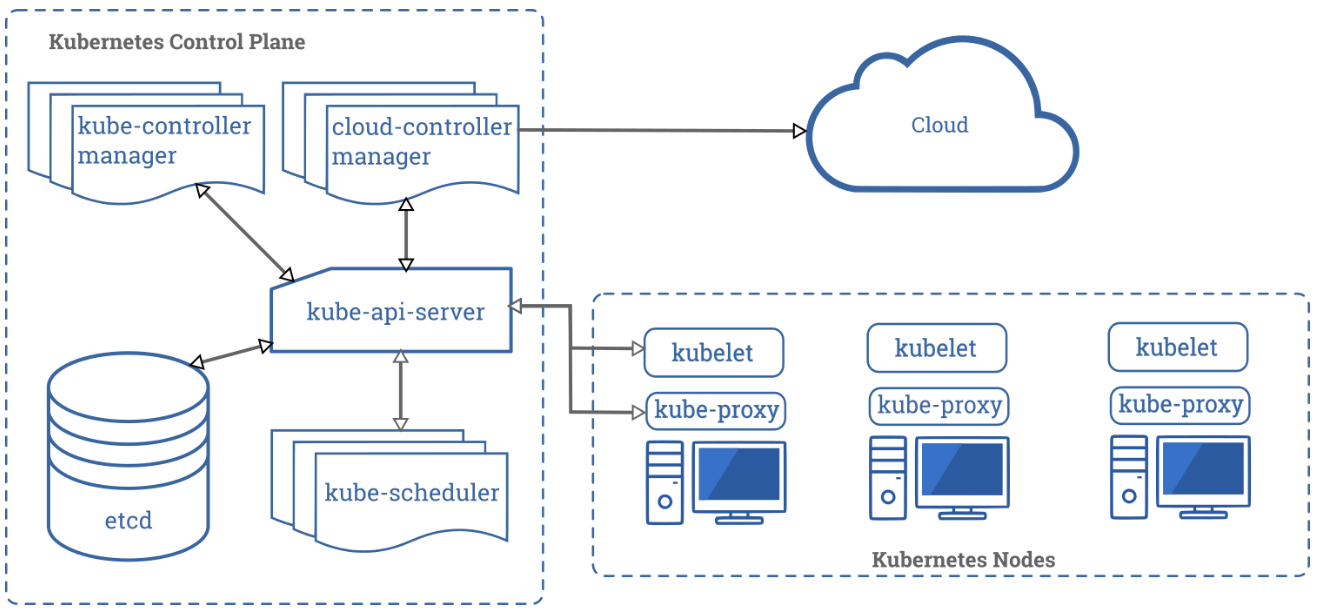
\includegraphics[width=0.95\textwidth, angle=0]{kubernetes-architecture.png}
 	\caption[Komponenty Kubernetes]{Komponenty Kubernetes}\label{fig:architecture}
\end{figure}

\subsubsection{Pod}
% https://medium.com/@aykanferhat/running-our-first-container-on-kubernetes-80041d659633
Pod je základní stavební jednotka Kubernetes. Je to balíček kontejnerů nebo též samostatný kontejner, který je specifikován v deploymentu a Kubernetes se o něj mají starat. Pro představu je zde obrázek, z čeho se pod skládá. Takových podů může být na jednom nodu několik. To jak se rozhodneme zabalit naši aplikaci do podů je čistě na tom, jak se rozhodneme. Abychom však neporušovali konvence tzv. service architektury. Musíme do jednoho podu dávat služby pouze takové, které dávají smysl. Pro příklad nebudeme do jednoho podu balit databázi s webovým UI. Při škálování by se totiž nejen že replikovala aplikace ale i databáz.  

\begin{figure}[!ht]
	\centering
 	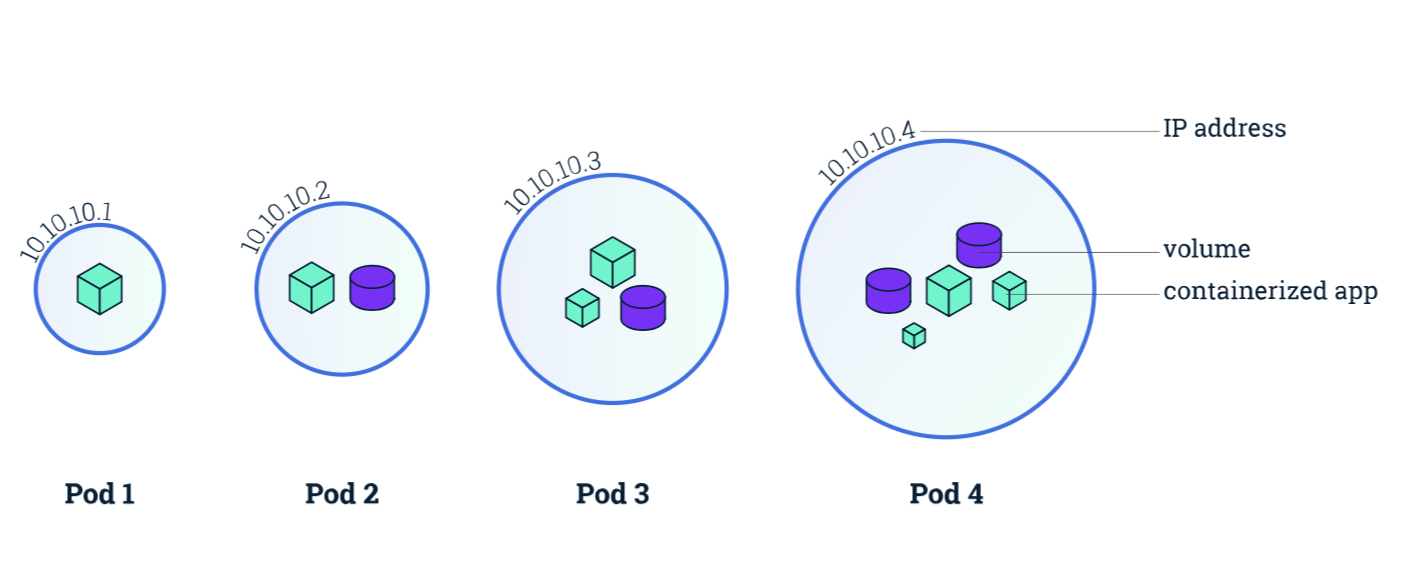
\includegraphics[width=0.8\textwidth, angle=0]{kubernetes-pod.png}
 	\caption[Kubernetes Pod]{Z čeho se skládá pod.}\label{fig:pod}
\end{figure}



\subsubsection{Control Plane}

Součásti Control plane řídí a rozhodují co se stane s klastrem, např. řídí plánování, detekci a odpovědi klastru na události, jako jsou start nového podu pokud není splněn požadovaný stav. 

Komponenty Control plane mohou být spuštěny na jakémkoliv počítači v klastru. Pro jednoduchost jsou však skripty napsané tak, aby tyto komponenty byly spuštěny na jednom počítači. Samotná aplikace je pak směřována mimo tento počítač. 

% https://github.com/etcd-io/etcd
\begin{itemize}

	\item \textbf{kube-apiserver}: Tato komponenta poskytuje API uživateli. Je to front end pro Control plane. Hlavní implementací je kube-apiserver, ten je navržen, aby se dokázal horizontálně škálovat, to znamená, že se dokáže replikovat do více instancí. Můžeme tedy spustit více instancí a balancovat provoz. 

	\item \textbf{etcd}: Skládá se z vysoce dostupné databáze s klíčem a hodnotou pro Kubernetes a všechna klastrová data. Její důležité vlastnosti jsou: jednoduchost, bezpecnost, rychlost, spolehlivost. 

	\item \textbf{kube-scheduler}: Tato komponenta kontroluje a vytváří nové pody, pro které zatím nebyl přiřazen žádný node. Je odpovědná za přiřazení takového podu na nějký node podle požadavků. Vždy musí brát v potaz zdroje, které jsou nutné, hardwarové a softwarové vazby, affinity a anti-affinity specifikace, kde jsou uložena data, vnitřní vytížení a časové termíny.

	\item \textbf{kube-controller-manager}: V této komponentě je spuštěn proces pro kontrolu klastru. Skládá se z více částí, které jsou zkompilovány do jednoho programu aby mohly běžet v jednom procesu, který se o vše stará. A stará se o následující:
	\begin{enumerate}

		\item \textbf{Node Controller}: Odpovědný za upozonění pokud jeden z nodů přestane odpovídat.

		\item \textbf{Replication Controller}: Odpovědný za dodržování správného počtu spuštěných aplikací v klastru. Pokud tedy část aplikace spadne je odpovědný za start nové instance.

		\item \textbf{Endpoints Controller}: Přidá nová uzly, nebo-li připojí služby a pody do klastru po jejich spuštění. 
	
		\item \textbf{Service Account a Token Controllers}: Vytváří výchozí účty a přístupové tokeny k API pro nové namespacy. 
	\end{enumerate}
	
	%https://kubernetes.io/docs/tasks/administer-cluster/running-cloud-controller/
	% https://github.com/kubernetes/cloud-provider/blob/master/cloud.go
	\item \textbf{cloud-controller-manager}: Tento daemon dovoluje připojit cloudové služby. Byl vytvořen pro možnost oddělení cloudových vývojařů od zdrojového kódu Kubernetes. cloud-control-manager je možné připoji k jakému koliv poskytovateli, který implementuje cloudprovider.interface.
\end{itemize}

\subsection{Komponenty nodu}

Node, jak je již uvedeno výše, je v podstatě stroj, který je připojen do klastru. Na tomto nodu mohou běžet pody, což je balík kontejnerů. Níže je popsáno z čeho se tento node skládá a co na něm musí běžet, aby Kubernetes správně operovalo.

\subsubsection{Kubelet}

Je agent zajišťující běh všech kontejnerů v daném podu. Kubelet převezme množinu požadavků na daný pod, tzv. PodSpecs a zajistí, že všechny kontejnerz popsány v těchto specifikacích jsou spuštěné a odpovídají na health checky. 

\subsubsection{Kube-Proxy}

Je síťová proxy, která běží na každém nodu. Spravuje síťová pravidla. Zajišťuje tak komunikaci mezi jednotlivými pody a nody uvnitř klastru. Používá szstémovou vrstvu na filtrování paketů, pokud je dostupná, jinak forwarduje provoz za pomoci svých prostředků. Níže znázorněno na obrázcích.
% https://kubernetes.io/docs/concepts/services-networking/service/
\begin{figure}[!ht]
	\centering
 	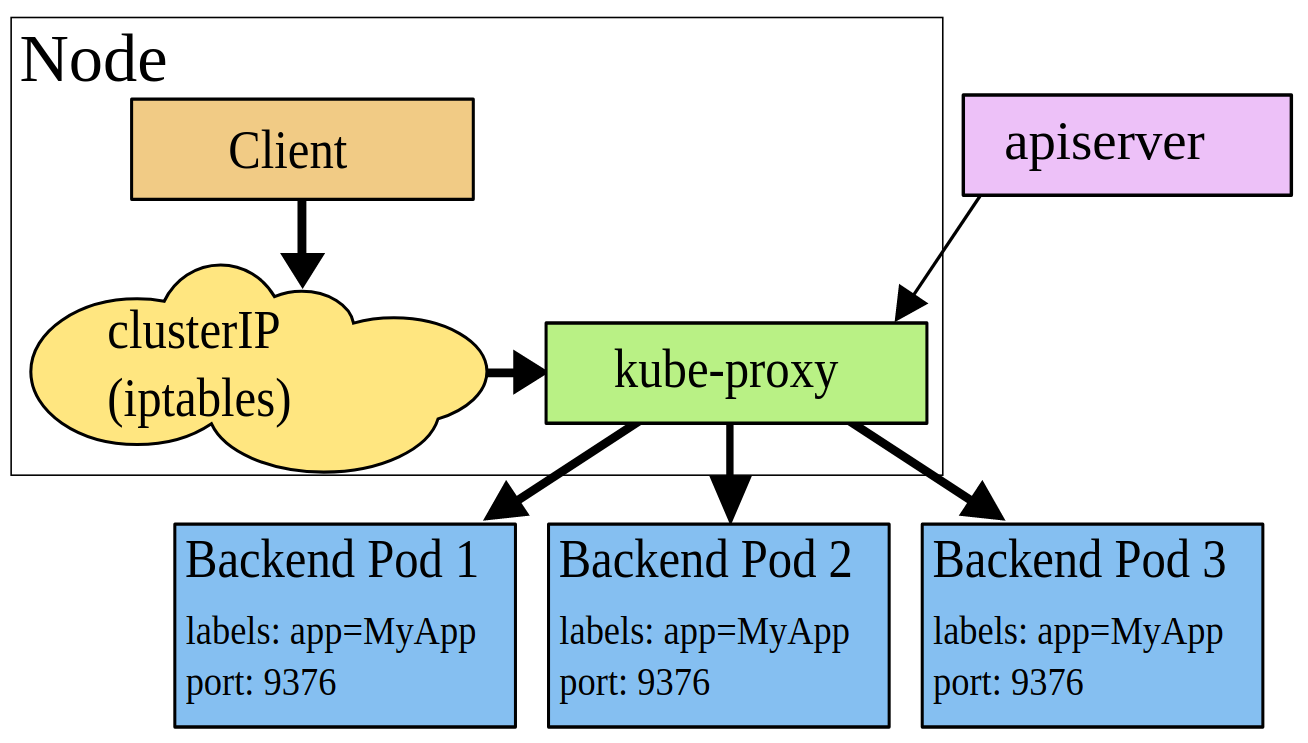
\includegraphics[width=0.8\textwidth, angle=0]{kubernetes-proxy.png}
 	\caption[Kubernetes proxy v user space módu]{Kubernetes proxy - User space proxy mode}\label{fig:usmp}
\end{figure}

\begin{figure}[!ht]
	\centering
 	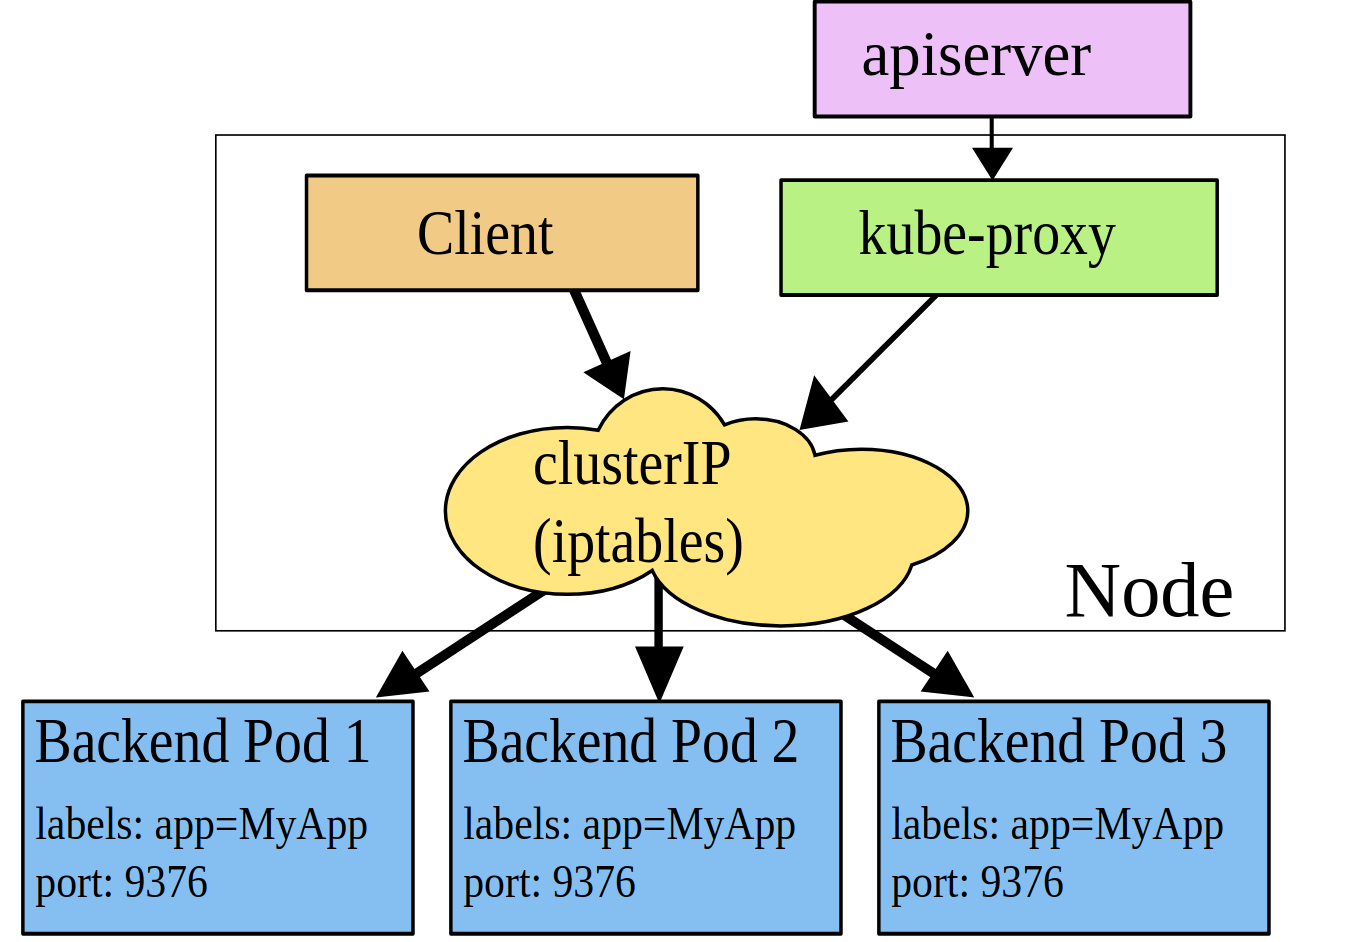
\includegraphics[width=0.8\textwidth, angle=0]{kubernetes-proxyip.png}
 	\caption[Kubernetes proxy fungující s iptables]{Kubernetes proxy - iptables proxy mode}\label{fig:iptpm}
\end{figure}



